\documentclass{book}

\usepackage[utf8]{inputenc}
\usepackage[T1]{fontenc}
\usepackage[francais]{babel}
\usepackage{graphicx} 



\title{Classification d'images télévisées}
\author{\textsc{Farhad} - \textsc{Heybati}\\
\textsc{Youcef} - \textsc{Kacer}\\
\textsc{Martin} - \textsc{Provost}}
\date{9 May 2016}

\begin{document}
 
\maketitle

\tableofcontents

\frontmatter
\chapter{Introduction}
Ce document présente plusieurs méthodes d'extraction d'informations à partir d'images issues d'un débat télévisé.
Cela afin d'en effectuer une classification binaire en \og gros plan \fg{} ou \og large plan \fg{}.
Nous proposons dans un premier chapître de présenter les images exploitées, et les deux classes qui nous intéressent.
Dans une seconde partie, nous presentons les méthodes d'extraction d'informations utilisées.
Puis dans une troisième partie, les résultats obtenus.

\mainmatter
\chapter{Images exploitées}
\section{Corpus et labelisation}
Nous allons exploités un total de 2351 images prises à partir de la vidéo d'un débat télévisé \cite{ref} .
Nous avons exploité le fichier de transcription au format .trs \cite{ref} associé à cette vidéo, cela afin d'extraire les différents classes, et attribuer à chaque image sa classe.
En effet, le fichier de transcription fournit un total de 9 classes : \\


\begin{description} % listes descriptives

\item[$M$ :] La présentatrice est seule à l'écran
\item[$A$ :] La première intervenante est seule à l'écran
\item[$B$ :] La seconde intervenante est seule à l'écran
\item[$C$ :] Le premier intervenant est seul à l'écran
\item[$D$ :] Le second intervenant est seul à l'écran
\item[$ALL$ :] Les 5 personnes sont à l'écran
\item[$MULTI$ :] Entre 2 et 4 personnes sont à l'écran
\item[$INTRO$ :] Reportage d'introduction à l'écran
\item[$CREDITS$ :] Générique d'emission à l'écran\\

\end{description}

Par ailleurs, le fichier de transcription donne à chaque intervalle de temps, ce qui est à l'écran parmi les classes citées plus-haut. Moyennant, une conversion du fichier au format xml, on peut obtenir
le tableau suivant :

\begin{table}[H]
\begin{center}
\begin{tabular}{|c|c|c|}
\hline
\begin{bf}classe\end{bf} & \begin{bf}debut (s)\end{bf} & \begin{bf}fin (s)\end{bf} \\
\hline
$CREDITS$	& 0 & 11.36 \\
\hline
$INTRO$   & 11.36	& 84.64 \\
\hline
$M$	& 84.64	& 95.12 \\
\hline
$ALL$	& 95.12	& 103.2 \\
\hline
$A$	& 103.2	& 112.2 \\
\hline
$M$	& 112.2	& 115.24 \\
\hline
\vdots & \vdots &\vdots \\
\hline
$M$	& 2334.12 & 2340 \\
\hline
$ALL$	& 2340 & 2340.76 \\
\hline
$CREDITS$	& 2340.76 & 2349.72 \\
\hline
\end{tabular}
\end{center}
\caption{Table de correspondance classes/intervalle de temps}
\label{Table correspondance classe/temps}
\end{table}
\clearpage

Les 2351 images étant prises à une seconde d'intervalle tout le long de la vidéo, on peut automatiquement labélisé celles ci via la table de
correspondance \ref{Table correspondance classe/temps}.
Ci-après, nous présentons quelques images pour chacune des 9 classes :
\begin{figure}[H]
\begin{center}
\includegraphics[scale=0.3]{../data/00000089.jpg}
\includegraphics[scale=0.3]{../data/00000159.jpg}
\includegraphics[scale=0.3]{../data/00000176.jpg}
\end{center}
\caption{image de classe $M$}
\label{classeM}
\end{figure}

\begin{figure}[H]
\begin{center}
\includegraphics[scale=0.3]{../data/00000105.jpg}
\includegraphics[scale=0.3]{../data/00000106.jpg}
\includegraphics[scale=0.3]{../data/00000107.jpg}
\end{center}
\caption{image de classe $A$}
\label{classeA}
\end{figure}

\begin{figure}[H]
\begin{center}
\includegraphics[scale=0.3]{../data/00000147.jpg}
\includegraphics[scale=0.3]{../data/00000148.jpg}
\includegraphics[scale=0.3]{../data/00000149.jpg}
\end{center}
\caption{image de classe $B$}
\label{classeB}
\end{figure}

\begin{figure}[H]
\begin{center}
\includegraphics[scale=0.3]{../data/00000165.jpg}
\includegraphics[scale=0.3]{../data/00000166.jpg}
\includegraphics[scale=0.3]{../data/00000167.jpg}
\end{center}
\caption{image de classe $C$}
\label{classeC}
\end{figure}

\begin{figure}[H]
\begin{center}
\includegraphics[scale=0.3]{../data/00000288.jpg}
\includegraphics[scale=0.3]{../data/00000289.jpg}
\includegraphics[scale=0.3]{../data/00000290.jpg}
\end{center}
\caption{image de classe $D$}
\label{classeD}
\end{figure}

\begin{figure}[H]
\begin{center}
\includegraphics[scale=0.3]{../data/00000179.jpg}
\includegraphics[scale=0.3]{../data/00000203.jpg}
\includegraphics[scale=0.3]{../data/00000239.jpg}
\end{center}
\caption{image de classe $ALL$}
\label{classeALL}
\end{figure}

\begin{figure}[H]
\begin{center}
\includegraphics[scale=0.3]{../data/00000213.jpg}
\includegraphics[scale=0.3]{../data/00000251.jpg}
\includegraphics[scale=0.3]{../data/00000310.jpg}
\end{center}
\caption{image de classe $MULTI$}
\label{classeMULTI}
\end{figure}

\begin{figure}[H]
\begin{center}
\includegraphics[scale=0.3]{../data/00000013.jpg}
\includegraphics[scale=0.3]{../data/00000024.jpg}
\includegraphics[scale=0.3]{../data/00000041.jpg}
\end{center}
\caption{image de classe $INTRO$}
\label{classeINTRO}
\end{figure}

\begin{figure}
\begin{center}
\includegraphics[scale=0.3]{../data/00002344.jpg}
\includegraphics[scale=0.3]{../data/00002348.jpg}
\includegraphics[scale=0.3]{../data/00002350.jpg}
\end{center}
\caption{image de classe $CREDITS$}
\label{classeCREDITS}
\end{figure}

\section{Classification binaire}

Par la suite, nous allons nous resteindre à seulement deux classes définies comme suit :\\
\begin{description} % listes descriptives
\item[$G$ :] \og Gros plan \fg{} (une seule personne est à l'ecran)
\item[$L$ :] \og Large plan \fg{} (au moins deux personnes sont à l'écran)\\
\end{description}


Les classes $G$ et $L$ peuvent s'exprimer en fonction des 9 classes comme suit :\\

\begin{description} % listes descriptives
\item[$G$ :] $M$ | $A$ | $B$ | $C$ | $D$
\item[$L$ :] $ALL$ | $MULTI$\\
\end{description}


Nous avons donc deux classes d'images $G$ et $L$ dont voici plusieurs exemples :\\

\begin{figure}[H]
\begin{center}
\includegraphics[scale=0.2]{../data/00000089.jpg}
\includegraphics[scale=0.2]{../data/00000105.jpg}
\includegraphics[scale=0.2]{../data/00000147.jpg}
\includegraphics[scale=0.2]{../data/00000165.jpg}
\includegraphics[scale=0.2]{../data/00000288.jpg}
\end{center}
\caption{image de classe $G$ (gros plan)}
\label{classeG}
\end{figure}

\begin{figure}[H]
\begin{center}
\includegraphics[scale=0.2]{../data/00000336.jpg}
\includegraphics[scale=0.2]{../data/00000394.jpg}
\includegraphics[scale=0.2]{../data/00000458.jpg}
\includegraphics[scale=0.2]{../data/00000474.jpg}
\includegraphics[scale=0.2]{../data/00000625.jpg}
\end{center}
\caption{image de classe $L$ (large plan)}
\label{classeL}
\end{figure}

Par la suite, nous allons expliciter différentes manières d'extraire de l'information afin de pouvoir discriminer les images de classe $G$
, des images de classe $L$.

\chapter{Extraction d'information}
\section{Extraction de contours}
\section{Extraction de teinte}
\section{Histogramme orienté du gradient}

Cette méthode consiste à extraire l'information local de contours. Sa première utilisation a consisté en 
la détection de piétons \cite{hog}. Pour une image donné, le vecteur descripteur des \begin{itshape}HOG\end{itshape} est la concaténation
d'histogrammes de l'amplitude du gradient (en fonction de l'orientation) pris sur un découpage de l'image:
\begin{figure}[H]
\begin{center}
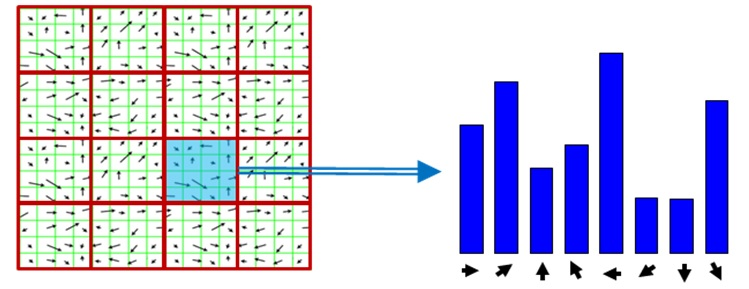
\includegraphics[scale=0.5]{hog.jpg}
\end{center}
\caption{construction d'un histogramme orienté du gradient \cite{hog2}}
\label{hog}
\end{figure}

On peut espérer que ces descripteurs s'adaptent bien à notre problème. En effet, les epaules des intervenants à gauche 
et à droite de l'image sont des contours descriminants pour la classe $G$ (gros plan). D'autre part, les gros plans ont fond uniforme, 
ce qui donnera beaucoup de gradient nul, et donc un descripteur \begin{itshape}sparse\end{itshape}

\begin{figure}[H]
\begin{center}
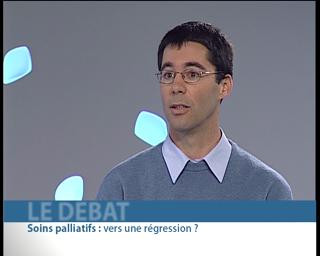
\includegraphics[scale=0.3]{hog_exemple.jpg}
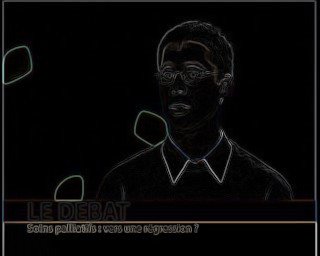
\includegraphics[scale=0.3]{hog_exemple_contour.jpg}
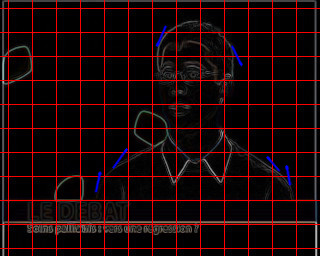
\includegraphics[scale=0.3]{hog_exemple_gradient.jpg}
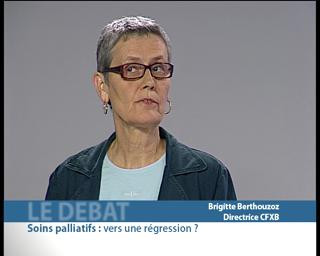
\includegraphics[scale=0.3]{hog_exemple2.jpg}
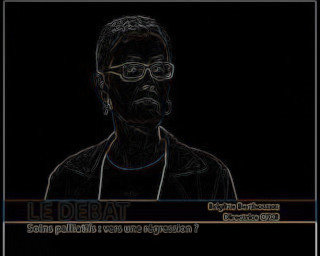
\includegraphics[scale=0.3]{hog_exemple2_contour.jpg}
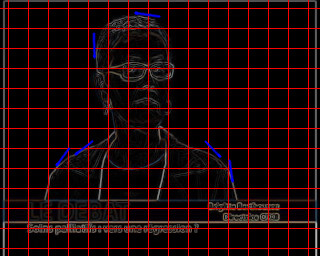
\includegraphics[scale=0.3]{hog_exemple2_gradient.jpg}
\end{center}
\caption{histogramme orienté du gradient pour les gros plans (classe $G$)}
\label{hog_classeG}
\end{figure}

\section{Reseaux de neurones à convolution pré-entrainé}

Cette méthode consiste à extraire les descripteurs produits par un réseau de neurones à convolution déjà entrainé.
En effet, en récupérant la sortie de l'avant-dernière couche, on obtient la transformation finale haut-niveau de l'image, avant la couche de classification.
Cette technique est connu sous le nom de \begin{itshape}Transfer Learning\end{itshape} \cite{DBLP:journals/corr/YosinskiCBL14} et a fait ses preuves dans 
le cas de réseaux de neurones entrainé sur la base d'images \begin{itshape}ImageNet\end{itshape} \cite{imagenet_cvpr09}.
Cette base de près de 10 millins d'images, contient une multitude de classes (animaux,ustensiles,humains,...) organisé hiérarchiquement, et on peut espérer que les gros plans
(classe $G$) correspondent à l'une des ses classes,et de même pour les images plan large (classe $L$), de telle sorte qu'on puisse ensuite séparer les descripteurs via un classifieur
 supervisé.

\chapter{Résultats}
\section{Extraction de contours}
\section{Extraction de teinte}
\section{Histogramme orienté du gradient}
Nous avons extrait les descripteurs \begin{itshape}HOG\end{itshape} pour chacune des images de classe $G$ et $L$, en utilisant une fenêtre glissante de taille $32x32$ avec un overlap. Puis, nous 
leur avons appliquer différent classifieurs supervisés. Nous avons découpé le set de descripteurs en deux sous-ensembles représentant 70\% du total pour l'entrainement, 
30\% pour le test. Les resultats de classification sont illustrés dans la table.
\section{Reseaux de neurones à convolution pré-entrainé}
Nous avons utilisé le code \begin{itshape}Overfeat\end{itshape} \cite{DBLP:journals/corr/SermanetEZMFL13}, récupéré par clonage du dépôt 
Github correspondant \cite{overfeat}, pré-entrainé sur la base \begin{itshape}ImageNet\end{itshape} \cite{imagenet_cvpr09}.
Nous avons extrait les descripteurs pour chacune des images de classe $G$ et $L$ pour leur appliquer différent classifieurs
 supervisés. Nous avons découpé le set de descripteurs en deux sous-ensembles s 70\% du total pour l'entrainement, 30\% pour le test.
 Les resultats de classification sont illustrés dans la table.

\backmatter

\listoftables

\listoffigures

\bibliographystyle{alpha}
\bibliography{biblio}

\end{document}